\documentclass[main.tex]{subfiles}
% \nomenclature[A]{GPR}{Ground Penetrating Radar}%

\begin{document}
\chapter{Testing}
\chaplabel{testing}
Tests were conducted to ensure that each subsystem was functioning correctly. Quad bike testing included initial testing of electronic components with subsequent stages added for total system integration to ensure that the autonomous navigation objective was complete.
(\textcolor{red}{Need to explain testing for GPR and metal detector and integrated systems testing})

\section{Test plan ???}
\textcolor{red}{Maz wants a new section that explains why we are doing the tests we are doing, and what the structure of the overall test plan is. \textbf{Within each subsequent section, start with aims of test, cover the test plan/requirements (need to include schematics and tables), discuss the results and talk about the relevance to the project objectives}}

\section{Sensor testing}
The completed tests and its procedure is discussed and includes details of the target objects buried and scanned with the AMDS metal detector and SIROPULSE II GPR. The results from these tests are provided with further analysis of how the data is used. 

\subsection{Test procedure}
\seclabel{testProcedure}
The purpose of sensor testing was to confirm that the algorithm produced in the detailed design section functioned correctly, and to gather further data points in order to build up a database for target identification. The testing plan outlined in (\Chapref{testProcedureApp}) provides detailed information regarding the overall goals and objectives for each test completed and the procedures for testing with the two sensors. 

In order to identify landmine signatures, replica (dummy) landmines loaned from the DSTG were used. These dummy landmines have similar characteristics to real landmines, including size, material composition and density. The three dummy landmines used were an metallic anti-tank mine (AT), a high metal content anti-personnel mine (APM) and a low metal content anti-personnel mines (APC) as seen in \Figref{dummy}. The APM contains greater than 10 grams of metal, and the APC contains less than 10 grams of metal \parencite{chant2005dsto}. The insides of the replica landmines are filled with paraffin wax and nylon to simulate the properties of real landmines when used with electromagnetic induction equipment \parencite{chant2005dsto}. These landmines are expected to have a density between 1.6 to 1.8 g/cm$^3$, whereas, the soil is expected to have a density between 1.0 to 2.5 g/cm$^3$ \parencite{das2002soil}.		
\begin{figure}[ht]
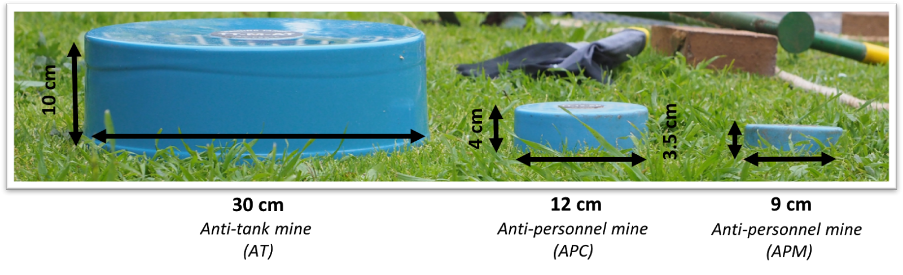
\includegraphics[width=0.9\textwidth]{5-Testing/dummy.PNG}
\centering
\caption{Landmine replicas used for testing }
\figlabel{dummy}
\end{figure}

The dummy landmines were compared to several clutter objects present, representing false positives that could be found in conflict areas. The clutter objects used in the test are shown in \Figref{clutter}. These can be categorised as metallic (steel, aluminium, tin, lead) and non-metallic content (rocks, plastic, wood). Some of these objects were used as they were expected to have similar properties and signatures to real landmines. Identifying these objects using both sensors and producing the metrics defined in detailed design will then lead to a quantifiable range of outputs to classify both dummy landmines and clutter objects.

\begin{figure}[ht]
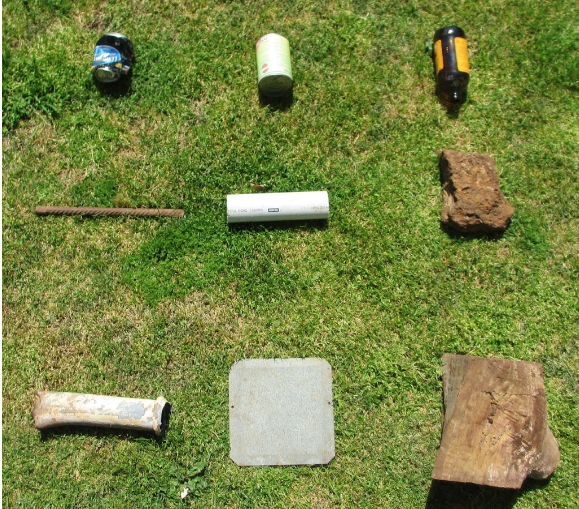
\includegraphics[width=0.6\textwidth]{5-Testing/clutter.PNG}
\centering
\caption[Clutter objects buried in the ground]{Clutter objects buried in the ground, from top left to bottom right: aluminium, tin can, glass bottle, steel rebar, pvc pipe, large rock, lead pipe, galvanised metal plate and wooden stump}
\figlabel{clutter}
\end{figure}

The dummy landmines were buried at three different depths, 2.5 cm, 7.5 cm and 15 cm respectively, as these depths are used by the DSTG in their standardised landmine detection test procedures. The depths are used to identify and compare the strength of the reflected signals for both metal detector and GPR as landmines are buried at varying depths. The clutter objects were buried at only 7.5 cm depth for an average comparison between the two depths. 

The central transmission frequency of 1.4 GHz was selected for the GPR antennae head. This frequency was found to provide a balance between detection depth and signal resolution and increase signal to noise ratio in comparison to both 800 MHz and 2 GHz GPR antennae. Data was recorded at all four available frequencies for the metal detector.

The testing was completed by scanning over each target column in the grid 12 times, six forwards and six backwards in order to produce large dataset. The data from both metal detector and ground penetrating radar were collected and processed with the algorithms defined in the detailed design chapter. Discussion and analysis of the results from the test is provided in the next section. 

\subsection{Results}
Analysis of the results from the main test will enable confirmation of unique metrics for both metal detector and ground penetrating radar. Feature analysis will be completed independently due to the different output metrics produced by the different signals. 

\subsubsection{Metal detector}
The phase angle and signal magnitude are the two main characteristics that were investigated. The metal detector data processed was analysed based on the magnitude and phase angle variation with target depth, and the phase angle variation versus the signal magnitude.

\Figref{phaseDepth} shows the phase angle result of the objects at varying depths. It is found that the phase angle is consistent across the three operating depths, as expected based on the results of the completed outdoor preliminary tests. The average phase angle for both anti-tank and high metal content anti-personnel mine were positive 25 degrees and negative 50 degrees, respectively. From the nine clutter objects tested, only five signatures may be compared with these two landmines. Based on the calculated results, the only object with phase angles closely similar to the anti-tank mine is the thin galvanised plate with an average phase angle of positive 16 degrees. However, the plate’s signature is differentiable from the actual anti-tank mine using the second metric. 
\begin{figure}[ht]
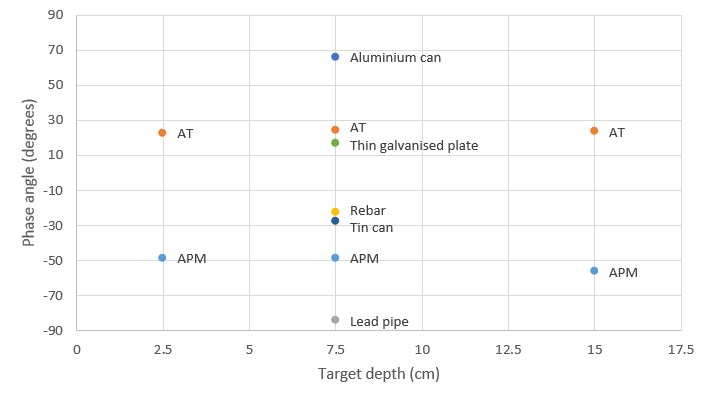
\includegraphics[width=0.9\textwidth]{5-Testing/phaseDepth.PNG}
\centering
\caption{Phase angle variation with target depth }
\figlabel{phaseDepth}
\end{figure}

Upon inspection of the graph (\Figref{magDepth}), signal magnitude with varying depths, the two landmines provide distinguishable magnitudes when compared with the other clutter objects. This graph also confirms that there is a differentiation between the anti-tank mine and the thin galvanised plate. This information can then be used to increase the probability of detection between these two objects. 

The anti-personnel mine and steel rebar have two similar signatures, with an average signal magnitude of 7.9e4 and 6.9e4, respectively. This factor provides an increase in false positive detection rate for the anti-personnel mine if they are both detected simultaneously. However, this false positive detection rate is reduced by analysing the phase angle of the object shown in the previous \Figref{phaseDepth}.

\begin{figure}[!ht]
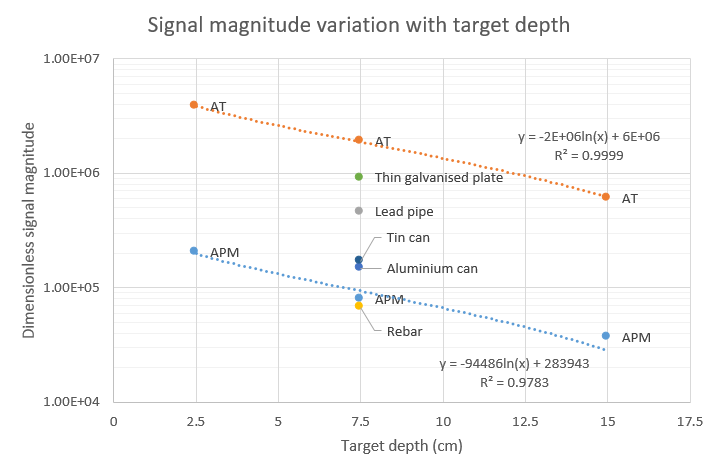
\includegraphics[width=0.9\textwidth]{5-Testing/magDepth.PNG}
\centering
\caption{Signal magnitude variation with target depth }
\figlabel{magDepth}
\end{figure}

When the phase angle is plotted against the signal magnitude (\Figref{phaseMag}), it was found that the phase angle calculated was consistent with a variation in magnitude of signals and thus, can be deduced that the phase angle is independent of the depth or magnitude. From this point, a confidence interval may be given to a phase angle value and confirmed with the corresponding signal magnitude range. 

A noticeable result for this plot is that the thin galvanised plate was within the signatures of the anti-tank mines. This means that it may be detected by the metal detector as an anti-tank mine and increase the false positive rate. 

\begin{figure}[ht]
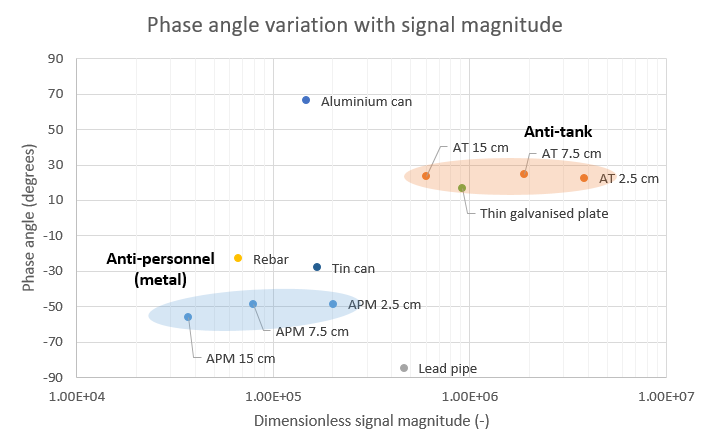
\includegraphics[width=0.9\textwidth]{5-Testing/phaseMag.PNG}
\centering
\caption{Phase angle variation with signal magnitude}
\figlabel{phaseMag}
\end{figure}

In summary, the anti-tank and anti-personnel mines produced distinguishable metrics for both phase angle and signal magnitude. However, as tabulated below (table xx), each metric can produce at least one false positive out of eleven objects, giving an approximate percentage confidence of detection of 90\%. It is possible to increase this probability of detection as one metric can confirm the other. The  thin galvanised plate can be identified and confirmed based on its magnitude calculation than its phase angle calculation. Similarly, the rebar can be identified with its phase angle calculation than its magnitude calculation as highlighted in \Tabref{mdMetrics}. Confirmation of the GPR feature width and depth may also increase this percentage confidence and will be discussed in the following subsection.

\begin{table}[ht]
\centering
\caption{ Summary of the false positive detection for metal detector metrics}
\tablabel{mdMetrics}
\begin{tabular}{lll}
\toprule
Object & Phase angle & Magnitude \\ \midrule
All APM & APM & APM \\
All AT & AT & AT \\
All APC & APC & APC \\
Thin galvanised plate & \textbf{AT} & Thin galvanised plate \\
Wood & None & None \\
Rock & None & None \\
PVC pipe & None & None \\
Glass bottle & None & None \\
Tin can & Tin can/Rebar & Tin can/Aluminium can \\
Aluminium can & Aluminium can & Aluminium can/tin can \\
Rebar & Rebar/Tin can & \textbf{APM} \\
Lead pipe & Lead pipe & Lead pipe\\ \bottomrule
\end{tabular}
\end{table}

\subsubsection{Ground penetrating radar}
The ground penetrating radar results are analysed based on the feature width and feature depth variation with target depth, and feature depth variation with feature width. 

\Figref{featureWidth} shows the  feature width plotted against the target depth, where AT is clearly distinguishable for all three depths. It also shows that both APC and APM have almost identical signals at depths of 2.5 and 7.5 cm. A number of clutter objects (glass bottle, PVC pipe and tin can) also have similar feature widths to the APM and APC at 7.5 cm, making it difficult to identify the mines. 

\begin{figure}[ht]
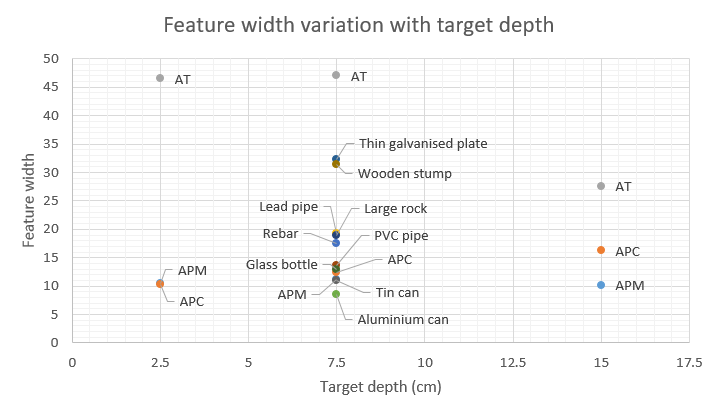
\includegraphics[width=0.9\textwidth]{5-Testing/featureWidth.PNG}
\centering
\caption{Feature width variation with target depth}
\figlabel{featureWidth}
\end{figure}

The results for the feature depth (\Figref{featureDepth}) are quite similar to the feature width at the target depth of 7.5cm. The characteristics and false positive rates are high for both APC and AT where the feature depth was similar to that of a large rock. However, this percentage probability can be differentiated using the feature width metric. Similarly, the feature width false detections for the tin can, glass bottle and PVC pipe can be differentiated using the feature depth.  The APM is distinguishable for all three depths for this plot.

\begin{figure}[!ht]
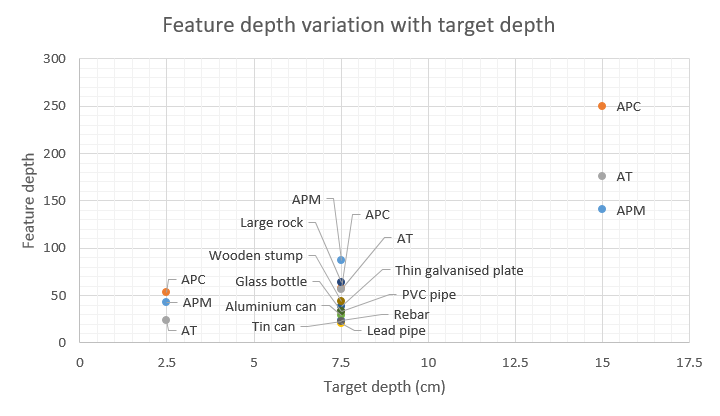
\includegraphics[width=0.9\textwidth]{5-Testing/featureDepth.PNG}
\centering
\caption{Feature depth variation with target depth}
\figlabel{featureDepth}
\end{figure}

When feature depth is plotted against the variation of feature width, all three mines have distinguishable features, with no clutter within their calculated ranges (\Figref{depthWidth}). Although it is differentiable, the clutter objects (aluminium can, tin can, glass bottle and PVC pipe) were found to be within close proximity to the signatures of both APM and APC at shallow target depths of 2.5 cm and 7.5 cm.

\begin{figure}[!ht]
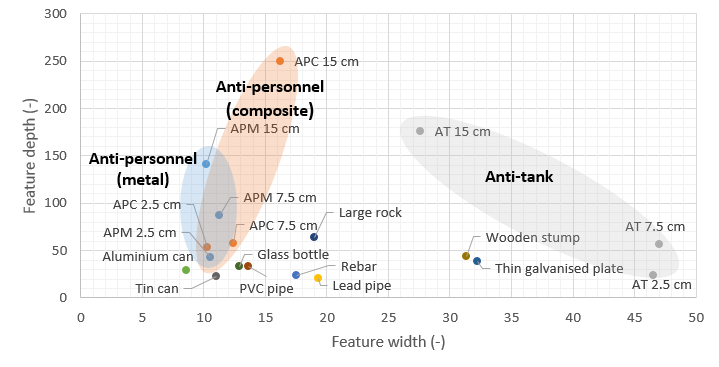
\includegraphics[width=0.9\textwidth]{5-Testing/depthWidth.PNG}
\centering
\caption{Feature depth variation with feature width}
\figlabel{depthWidth}
\end{figure}

The results from the plots in previous pages can be summarised in the table below (table xx). The AT is both distinguishable at all target depths using the feature width metric, and APM is distinguishable using the feature depth metric. As shown, the feature width has the lower percentage confidence at 73\%, with three objects (PVC pipe, glass bottle and tin can) out of eleven detected as an APC or APM. In comparison, the feature depth only produced one false positive, the large rock scanned as shown in \Tabref{gprMetrics}, out of the eleven objects scanned, which gives a 90\% confidence. From these results, the percentage confidence and objects can be confirmed without the use of metal detector metrics. 

\begin{table}[!ht]
\centering
\caption{Summary of the false positive detection for GPR metrics}
\tablabel{gprMetrics}
\begin{tabular}{lll}
\toprule
Object & Feature width & Feature depth \\ \midrule
All APM & APM/\textbf{APC} & APM \\
All AT & AT & AT/\textbf{APC} \\
All APC & APC/\textbf{APM} & APC/\textbf{AT} \\
Thin galvanised plate & Thin galvanised plate/Wood & Thin galvanised plate \\
Wood & Wood/Thin galvanised plate & Wood \\
Rock & Rock/Lead pipe & \textbf{APC/AT} \\
PVC pipe & \textbf{APC} & PVC pipe \\
Glass bottle & \textbf{APC} & Glass bottle \\
Tin can & \textbf{APM} & Tin can/Lead pipe \\
Aluminium can & Aluminium can & Aluminium can/PVC/Rebar \\
Rebar & Rebar & Rebar/PVC/Aluminium can \\
Lead pipe & Lead pipe/Rock & Lead pipe/Tin can\\ \bottomrule
\end{tabular}
\end{table}

\subsubsection{Discussion}
The results show that the algorithm can produce unique sets of data and is able to distinguish between the landmines and clutter objects. The metal detector output metrics produced consistent results and identified the AT and APM mines from both tests. In comparison, the GPR was able to distinguish between both metallic and non metallic objects, however, it was not as consistent as the metal detector output metrics and produced a higher rate of false positives. Further testing is required to be able to produce and analyse further data in order to reduce the false positive detection with the GPR algorithm. Regardless, the false positives can be reduced when the results from both sensors are combined using the sensor fusion algorithm discussed in detailed design.

The phase angle and magnitude output from the metal detector may be used independently to confirm metallic landmines and clutter objects. The phase angle data may be analysed first as this is independent of the target depth. If the algorithm detects it as a landmine, the magnitude is then used to confirm the object as shown in \Tabref{mdMetrics}. Similarly, the feature width for the GPR data may be analysed first, followed by a confirmation of the object using the feature depth. The data from these results are stored in a database to be used by the sensor fusion algorithm. The output metric values from the phase angle, magnitude, feature width and depth are then retrieved by the algorithm to be able to compare the current scans with the relevant values. This then produces a percentage confidence of the scanned object of being a landmine and sent wirelessly from the platform’s central computer system to the tablet device. The operator is then able to effectively decide to remove the object based on the data it receives from the processed data. 

\textcolor{red}{Seems to be some repetition here from the detailed design for sensor fusion. Need to discuss what some of the limitations of the tests were. Only a small number of clutter objects were used, clutter was only buried at one depth, if it was some other depth is might have led to more/less false positives, i.e. the current data set needs to be expanded on largely in order to make the detection algorithm more robust. The same type object would have a different signature if it was a different size, or in a different orientation - need to do more sensitivity testing, ideally in a controlled environment with the use of a test rig, allowing for repeated sweeps in an identical manner. \textbf{Some of these points could go in future work.}The results can't really be applied to any other scenarios, as both metal detector and GPR signals will look different in different soil types. Soil moisture was high, and the soil wasn't very clean (not layered nicely, rocks and things present), this may have had an effect on GPR results.Would be better to test in DSTG test lanes. Could not achieve real time processing, however the sensor fusion algorithm (still needs to be done) was tested with sample dara to simulate batch processing of results.}

\section{Positioning systems testing}
Individual positioning systems were tested and their errors analysed to be used in the Kalman Filter.
\textcolor{red}{expand?}
\subsection{GPS}
The primary function of the GPS in the positioning system was to correct for drift that may be present in the kinematic equations. For this purpose accuracy is very important however very small emphasis is placed on any error from noise, which is accounted for in the Kalman Filter. Testing of the GPS involved moving it around a known location over known distances. Two categories of testing were conducted, stationary tests and non-stationary tests. This was chosen as a result of the known differences in performance between the two.
\begin{figure}[ht]
\centerline{
\begin{tabular}{cc}
\subfloat[Non-stationary test]{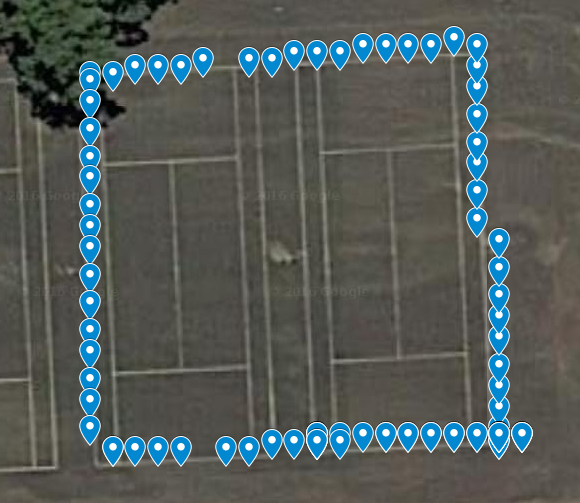
\includegraphics[height=0.4\textwidth]{5-Testing/nonStationaryGpsTest.png}} 
& \subfloat[Stationary test]{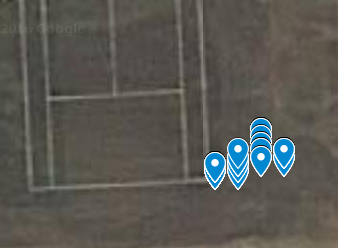
\includegraphics[height=0.4\textwidth]{5-Testing/stationaryGpsTest.png}}\\
\end{tabular}}
\caption{GPS tests}
\figlabel{gpsTests}
\end{figure}
The non-stationary test in \figref{gpsTests}a involved traversing the outer edge of two tennis courts, and during the stationary test the receiver was left sitting on the bottom right corner for 120 seconds. The GPS data was overlayed onto satellite imagery using Google Maps for better visualisation.

From the non-stationary test it is evident that when moving the GPS provides very accurate positional information, within 1 meters for the duration of the test. The stationary test revealed that the GPS suffers quite substantially from drift when sitting still, varying up to 6 meters from its actual position. For this reason, the GPS will only be to correct positional information in the Kalman Filter when the quad bike is at cruising speed, 5 km/hr.

\subsection{IMU}
To determine error present in the IMU it was correctly set on the quad bike and the engine started and throttled. The test procedure allowed the IMU to calibrate for 35 seconds before starting the engine. The engine idled for 45 seconds, then was throttled for 40 seconds before being turned off. The results are shown in \figref{yawTest} and \figref{yawTestZoomed}.
\begin{figure}[ht]
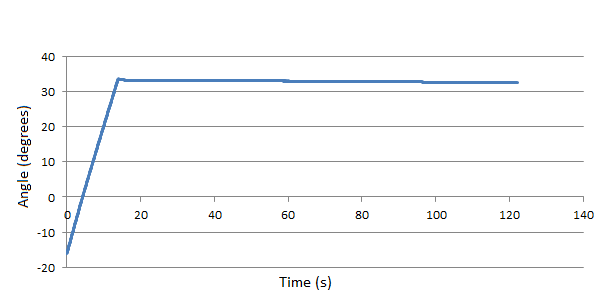
\includegraphics[width=1\textwidth]{5-Testing/yawTest.png}
\centering
\caption{Yaw test: calibration to 35 s, idle to 80 s, throttle to 120 s}
\figlabel{yawTest}
\end{figure}
\begin{figure}[ht]
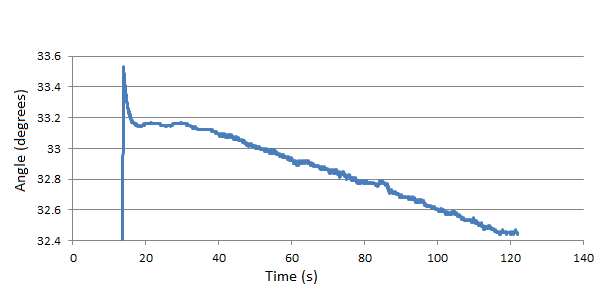
\includegraphics[width=1\textwidth]{5-Testing/yawTestZoomed.png}
\centering
\caption{Yaw test focused on angle from 32.4\degree to 33.6\degree}
\figlabel{yawTestZoomed}
\end{figure}
The IMU takes some time to calibrate, we can see from \figref{yawTestZoomed} that calibration is complete at $t=20s$. Over the remaining 15 seconds before the engine is started, the IMU holds its position almost perfectly. Over the remaining 85 seconds of the testing period, the IMU heading steadily decreases by a total angle of 0.7 degrees, a rate of $\frac{0.7\degree}{85\ seconds} = 0.008 \degree/s$. The same slope between idling and throttling showed that the error of the IMU did not depend on the rate of throttle of the engine, just if the engine was running or not.

Raw accuracy of the IMU was found by smoothly rotating the IMU 360\degree on a desk. Initial IMU readings were 87.3 degrees and the reading after the rotation was \~85.6 degrees, an error of $\frac{2\degree}{360\degree}$, or $0.056\degree/\degree$.

\subsection{Wheel encoder}
\seclabel{testingwheelencoder}
One of the primary functions of the wheel encoder was to give an accurate value for the distance travelled by the quad bike as well as it's operating speed. To test the encoder, data was compared with values obtained from the display unit on the quad bike. The two data sets are overlaid in \figref{encoder20x} and the instantaneous difference shown. Some sampling was necessary to reduce the noise present in the encoder data. 20x was found to be the best as it was able to smooth the noise while keeping accurate to the display speed. It was clear that the wheel encoder was doing an adequate job of representing the display speed. The second test was to evaluate how accurate the speed represented the actual distance travelled when integrated over time. \Tabref{encoderIntegration} shows the results of three tests. Test 1 and 2 consisted of manually spinning 10 revolutions of the quad bike wheel on its stand at a consistent speed. Test 3 involved 3 complete stops of the wheel throughout the 10 revolutions.

\begin{figure}[ht]
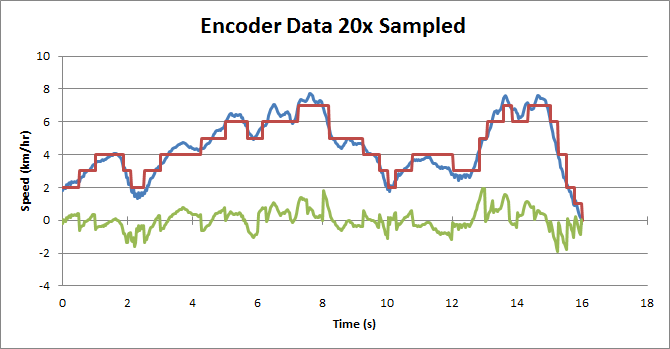
\includegraphics[width=1\textwidth]{5-Testing/encoder_data_20x_sampled.png}
\centering
\caption[Encoder speed reading compared with quad bike display]{Encoder speed reading compared with quad bike display with engine not running}
\figlabel{encoder20x}
\end{figure}

\begin{table}[ht]
\centering
\caption{Wheel encoder distance integration tests}
\tablabel{encoderIntegration}
\begin{tabular}{llll}
\toprule
                                   & Test 1 & Test 2 & Test 3 \\ \midrule
Rotations of the wheel:            & 10     & 10     & 10     \\
Number of readings:                & 7646   & 8843   & 19885  \\
Test time (seconds):               & 13.54  & 14.39  & 31.69  \\
Time interval (microseconds):      & 1770   & 1627   & 1594   \\
Circumference of wheel (m):        & 1.95   & 1.95   & 1.95   \\
Actual distance travelled (m):     & 19.5   & 19.5   & 19.5   \\
Calculated distance travelled (m): & 19.53  & 19.41  & 18.86  \\ \bottomrule
\end{tabular}
\end{table}

\textcolor{red}{TALKING ABOUT LIVE TESTS WITH ENGINE RUNNING HERE}
Tests for the encoder with the quad bike engine running were completed to see if the operation of the engine effected the speed output. \Figref{encoderEngine} shows the encoder readout for the engine tests. It can clearly be seen that there are large discrepancies in the speed outputs. It was found that the encoder support bracket vibrated against the encoder wheel resulting in large spikes in the speed reading. Upon firmly supporting the bracket, the noise was reduced but still present. A rubber damper and a support bracket was fixed to the encoder support and this reduced the noise level. However the reduction was still not adequate for the required accuracy. 

Speed tests were completed with the quad bike moving under its own power. The encoder readings were accurate however, large fluctuations were still inherent. A low pass filter was used to smooth out the data from the encoder leading to smoother and more accurate speed readings from the encoder. 
\begin{figure}[ht]
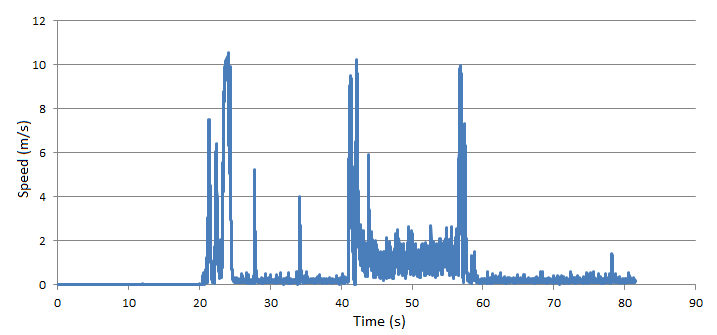
\includegraphics[width=1\textwidth]{5-Testing/Encoder_data_with_engine_running.png}
\centering
\caption[Encoder speed reading for various engine states]{Encoder speed reading when stationary and engine off (0s - 20s), engine idling (20s - 40s), engine throttling (40s - 60s), and while supporting the encoder bracket (60s - 80s)}
\figlabel{encoderEngine}
\end{figure}

\subsection{Integrated positioning system}
Testing for the positioning system was primarily undertaken inside the Virtual Platform (see \secref{detailedVP}). This was to ensure satisfactory performance of the system before live tests were undertaken. Simulated hardware components; GPS, IMU, and wheel the encoder, were used inside the Virtual Platform. Noise for each of the sensors was hard-coded into the software based on the values obtained from their respective tests.
\Figref{posError1} shows the x and y components of the distance error from the true value for the Kalman filtered position and the position from kinematic equations. The simulation consisted of a 25 degree right turn, 25 degree left turn, followed by a long straight beginning at the nine second mark. Due to the certain starting position of the quad bike the errors all begin at zero. When using the kinematic equations alone, the error grows due to the additive nature of the process. A diverging result occurs because the heading calculated through kinematics is not the true heading. When corrected with the IMU and GPS the Kalman position stabilises and the error peaks at approximately 0.4 meters, which is within specifications. \Figref{posError2} is a more realistic simulation, consisting of 2 x 90 degree right turns, a long straight, and 2 x 90 degree left turns to mimic a path that would be traversed throughout a set region. It is again apparent with the kinematic equations alone that error accumulates when a straight is encountered. When stabilised with the IMU and GPS units however, the resulting Kalman position remains accurate to within 0.2 meters, again within specifications.
\begin{figure}[ht]
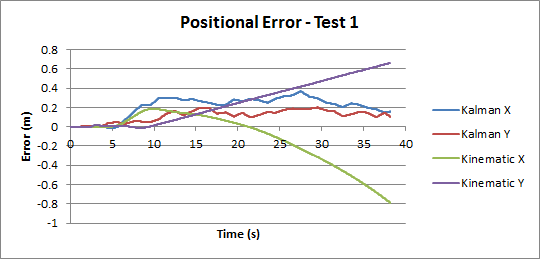
\includegraphics[width=\textwidth]{5-Testing/position_error_test_1.png}
\centering
\caption[Positioning system test 1]{Test 1: 25 degree right turn, 25 degree left turn, followed by long straight (from 9 seconds)}
\figlabel{posError1}
\end{figure}
\begin{figure}[ht]
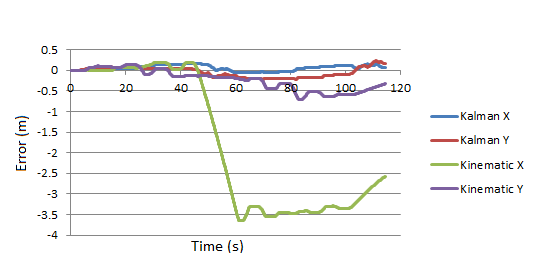
\includegraphics[width=\textwidth]{5-Testing/position_error_test_2.png}
\centering
\caption[Positioning system test 2]{Test 2: 2 x 90 degree right, long straight, 2 x 90 degree left, long straight} \figlabel{posError2}
\end{figure}

\section{Quad bike systems testing}
Preliminary testing of the quad bike subsystems were required to determine their working range, functionalities and integration. The systems tested were the brakes, steering, throttle, gear selector, wheel encoder, and positioning system. Additional safety systems were also tested to ensure they functioned as intended.
The relevant test cases were documented in separate files (\textcolor{red}{REFER TO APPENDIX??}).

\subsection{Brake testing}
The brakes were required to control the quad bike speed as well as to bring the platform to a complete stop when commanded or in the case of an emergency. This requires accurate knowledge of the brake position for the varying brake intensities. The maximum brake intensity was chosen as the point where the wheels were unable to be turned by hand. This was found through small 5 percent increments in the actuator extension until the wheels were unable to rotate. The time required for the brake actuator to go from nill brake to maximum was \textcolor{red}{MEASURED TO BE 3 SECONDS}. This coupled with a reduction in throttle would ensure that the quad bike is able to stop in the required distance of 60cm as specified in the constraints. During testing however, it was found that the throttle response was magnitudes faster in reducing the speed compared to the brake. the time delay between the brake being signalled to when it actually engages resulted  in the quad bike coasting to stop before they were engaged. The brake speed would and actuator choice were insufficient fro the required task and only proved useful in holding the position of the bike when on a slope. The quad was found to coast to a stop from operating speeds in 1.2 m, double the required stopping distance highlighted within the platform requirements.    \textcolor{red}{THIS LAST SENTENCE IS THE ACTUAL TEST THAT WE NEED TO DO - NOT COMPLETE YET}

\subsection{Gear testing}
The ability to control what gear the quad bike is in was essential to the control and navigation of the project. 36 testing cases were identified for the gear actuator setup. The actuator could lie in one of nine possible positions which were identified based on the system set-up and had three final positions, reverse, neutral and forwards as well as a null option for no actuator movement. \Chapref{gearTable} shows the final truth table.
The truth table indicates the gear selector code has full completion of the testing cases. The gear actuator should not move when the quad bike is in motion or when the throttle is engaged. This is to ensure that   A check in the software was implemented to achieve this. Testing of the system resulted in fine tuning requirements of the gear sensors. Initial tests resulted in the gear not mechanically being inserted even if it displayed it had on the quad bike display. This resulted in gearbox cogs grinding and the quad bike lurching forwards when the gear caught. Further tests lead to the adjustments in the Quad bike idle throttle position. Due to the idle being set too high, the centrifugal clutch would engage before the gear was properly selected leading to more gearbox grinding. Proper idle speeds resulted in smooth gear changes with no lurching or gearbox grinding.   \textcolor{red}{DO WE NEED MORE ON THIS?}

\subsection{Steering testing}
The steering of the quad bike was achieved through the use of a stepper motor. Upon power up, the position of the wheels would be the zero position and movement to the left or right dictated by the angle sent to the stepper motor. From the user manual for the quad bike the lock out angle for the steering was \textcolor{red}{24 degrees NEED TO CHECK}, a limit for the steering angle was placed at 23 degrees to ensure no structural damage occurred. 

Initial tests found that when the quad bike was on the support stand with the wheels free, the steering behaved as expected. However, when a resistive load was applied in the direction of the steering angle, the stepper motor would stop and reset. This would result in a incomplete steering angle as well as a new off centre zero position being selected by the stepper motor.  It was found that the required power for the stepper motor to operate to the required torque was 440W whereas the power supply in the quad bike was only able to supply 44W. Replacement of the power supply with one of the correct power requirements resulted in steering angle control under operational loads.

The accurate turning radius for the platform was required for the navigation software. The quad bike was allowed to travel forward from a marked position with the steering at full lock. Once a full circle was complete, the quad bike was turned off. The turn radius was measured to be 2.7m. This was within the turning circle range decided upon in the navigation software. A 30 degree steering limit was selected to allow for any small angle variations in the stepper motor from miss aligned initiations to minimise the risk to damaging steering linkages. Correct operation procedures with the initialisation of the quad bike would ensure that the extremes of the turning angle would not be met. 

\textcolor{red}{steering tests more?}

\subsection{Throttle testing}
The throttle is controlled via a rotational servo. Initial approximation of the throttle travel had the servo with zero throttle and maximum throttle at servo positions 75 and 150 respectively. With the engine warmed up, incremental increases resulted in an actual throttle response range to be calculated. Due to the circular sweep of the servo arm and some cable play, the minimum throttle position before a throttle response was found to be 97 and a maximum throttle position of 110 was chosen for the servo. This number was chosen due to the wheel speed in both forwards and reverse gears varying due to gearing and so the maximum servo position would be required for cruise speed in both directions of motion. A higher servo position than this would never be required for the chosen operating scenario.

live tests on the ground found that the added load on the drive-train only resulted in the quad bike moving forward when the throttle was set to 70 \% of the selected range of motion. once the quad bike started moving forwards and at operational speeds, a throttle of 60 \% was required to maintain the speed. Different terrains would offer different drag coefficients on the wheels leading to different throttle responses to overcome the initial drag to get the quad bike in motion. 

\section{Integrated system testing}

\end{document}